\documentclass{book}
\usepackage{titling}
\usepackage{multirow}
\usepackage{setspace}
\usepackage{makeidx}
\usepackage{tikz}
\usepackage{braket}
\usepackage{graphicx}
\usepackage{array}

\usepackage{qcircuit}
\usepackage{graphicx}

\usepackage{tabularray}
\usepackage{amsmath}
\usepackage{circuitikz}
\usepackage{amssymb}
\usepackage{setspace}
\usepackage{amsmath}
\usepackage{xepersian}
\settextfont{XB Zar}
\linespread{1.5}



\makeatletter
\def\TikzBipolePath#1#2{\pgf@circ@bipole@path{#1}{#2}}
\def\CircDirection{\pgf@circ@direction}
\makeatother

% TikZ libraries `calc` needed now to tweak bracket.
\usetikzlibrary{backgrounds,fit,decorations.pathreplacing,calc}

\begin{document}
\tableofcontents
\section{مقدمه}	
در عصر حاضر بواسطه‌ی رشد و توسعه‌ی نظریه‌ی اطلاعات کوانتومی و سرمایه‌گذاری های مالی و انسانی بسیار در این زمینه،‌شاهد افزایش تعداد علاقمندان به این حوزه هستیم. در این پا .....
\chapter{آشنایی با مفاهیم اولیه}
\section{کیوبیت}

یک کیوبیت\footnote{Qubit}، معادل یک واحد اطلاعات کوانتومی می‌باشد. این مفهوم معادل مفهوم کلاسیک بیت\footnote{Binary Bit} می‌باشد. به طور کلی هر کیوبیت حاوی دو بیت اطلاعات است. برای تبیین یک کیوبیت از خصوصیات سامانه های کوانتومی، بهره‌می‌بریم. کیوبیت یک سیستم کوانتومی با فضای دوبعدی است. برای تعیین این دوبعد می‌توان ا ز یکی از خصویات سامانه های کوانتومی استفاده کرد. 

برخلاف بیت ها که مقادیر ثابت 0 یا 1 را به خود می‌گیرند؛ یک کیوبیت می‌تواند در یک حالت «برهمنهی کوانتومی» باشد؛ این بدان معناست که یک کیوبیت بواسطه‌ی مشاهده ناظر به یکی از حالات 0 یا یک تبدیل شود. این مهم‌ترین مزیت استفاده از کیوبیت‌هاست. بیان ریاضی یک کیوبیت ،در حالت برهمنهی، به شرح زیر است:
\vspace{2cm}
$$
\left\{
\begin{array}{ll}
	  \vert \psi \rangle = \alpha\vert 0 \rangle + \beta\vert 1 \rangle \\
	  \alpha^2 + \beta^2 = 1
\end{array}
\right.
$$
\vspace{2cm}

\newpage
کت‌ها$\vert 0 \rangle$ و $\vert 1 \rangle$ بیانگر پایه‌های فضای 
محاسباتی\footnote{\lr{Computational Basis Vectors}} هستند؛ و مقادیر $\alpha^2$ و $\beta^2$ بیانگر احتمال وقوع هر یک از این حالات، در صورت مشاهده، می‌باشند.

نمایش بردار $\psi$ به شرح زیر است:
\begin{center}
\begin{tikzpicture}
	
	% Define the axes
	\draw[->] (-2,0)--(2,0) node[right]{$\vert 0 \rangle$};
	\draw[->] (0,-2)--(0,2) node[above]{$\vert 1 \rangle$};
	
	% Draw the vector
	\draw[black,-stealth] (0,0)--(1,2) node[anchor=south west]{$\vec{\psi}$};
	
	% Label the components of the vector
	\node[below] at (1,0) {$$};
	\node[left] at (0,2) {$$};
	
\end{tikzpicture}
\end{center}

در بسیاری از مواقع برای سهولت در محاسبات، عملگر‌ها و حالات کوانتومی به کمک ماتریس‌ها نمایش داده ‌می‌شوند. فرم ماتریسی هر یک از حالات ذکر شده در بالا به شرح زیر است:

\begin{equation}
	\vert 1 \rangle = \begin{pmatrix} 0 \\ 1 \end{pmatrix}
	\hspace{2cm}
	\vert 0 \rangle = \begin{pmatrix} 1 \\ 0 \end{pmatrix}	
\end{equation}

برای تعریف کیوبیت ها، راه های زیادی وجود دارد، حالات قطبش فوتون،‌اسپین الکترون،‌یا سطوح انرژی اتم،‌هریک می‌توانند تعیین کننده‌ی بردار‌های فضای کیوبیت باشند.

\section{bloch vector - computayional basis - fourier basis}
\section{گیت‌های کوانتومی}
گیت‌های کوانتومی\footnote{\lr{Quantum Gates}} یکی از اولین و ههم‌ترین اجزای‌ مدار‌های کوانتومی ‌می‌باشند. این گیت‌ها عملگر‌هایی با قابلیت اثر‌گذاری روی کیوبیت‌ها می‌باشند. با اعمال یک گیت کوانتومی بر روی یک یا چند کیوبیت، می‌توان تغییرات مدنظر خود را روی کیوبیت اعمال کرد. با کمک این گیت‌ها می‌توان باعث برهم‌نهی کوانتومی یا رمز‌گذاری داده در داخل یک یا چند کیوبیت شد.

\subsection{انواع گیت کوانتومی}
گیت‌های کوانتومی، دارای انواع مختلف گوناگونی می‌باشند. به طور کلی گیت‌های کوانتومی، عملگر‌هایی یکه و بازگشت‌پذیر می‌باشند. 
\subsection*{گیت هادامارد}
مهم‌ترین گیت کوانتومی،‌گیت هادامارد\footnote{\lr{Hadamard gate}} است. با اعمال اثر این گیت روی یک کیوبیت، آن کیوبیت به‌یک حالت برهم نهی‌ کوانتومی‌ گذار‌ می‌کند. به عبارت دیگر هر یک از زیرحالات این حالت برهم‌نهی، با احتمال یکسانی قابل رخ دادن‌ هستند. 
\vspace{1cm}
$$
H\ket{0} = \frac{1}{\sqrt{2}} (\ket{0} + \ket{1})
\hspace{2cm}
H\ket{1} = \frac{1}{\sqrt{2}} (\ket{0} - \ket{1})
$$
\vspace{1cm}

این گیت کوانتومی‌ به صورت خطی روی یک دسته‌ کت اثر مي‌کند. نمایش ماتریسی این گیت‌کوانتومی به شرح زیر است:
\begin{center}
	\[
	H = \frac{1}{\sqrt{2}}
	\begin{pmatrix}
		1 & 1 \\
		1 & -1
	\end{pmatrix}
	\]
\end{center}





\begin{align*}
	H |0\rangle = l\frac{1}{\sqrt{2}} \begin{pmatrix} 1 & 1 \\ 1 & -1 \end{pmatrix} \begin{pmatrix} 1 \\ 0 \end{pmatrix} \
	= \frac{1}{\sqrt{2}} \begin{pmatrix} 1 \\ 1 \end{pmatrix} \
	= \frac{1}{\sqrt{2}} (|0\rangle + |1\rangle)
\end{align*}

\begin{align*}
	H |1\rangle = l\frac{1}{\sqrt{2}} \begin{pmatrix} 1 & 1 \\ 1 & -1 \end{pmatrix} \begin{pmatrix} 0 \\ 1 \end{pmatrix} \
	= \frac{1}{\sqrt{2}} \begin{pmatrix} 1 \\ -1 \end{pmatrix} \
	= \frac{1}{\sqrt{2}} (|0\rangle - |1\rangle)
\end{align*}

این گیت کوانتومی، یک گیت بازگشت‌پذیر است؛ یعنی اگر این گیت روی یک حالت کوانتومی اثر کند؛‌ می‌تواند آن را از حالت برهمنهی خارج کند. 

برای اعمال این گیت کوانتومی، فقط به یک کیوبیت نیاز داریم. به اصطلاح این گیت،‌یک \lr{Single-Qubit Quantum gate} می‌باشد.

نمایش این گیت‌کوانتومی در مدار با علامت زیر است:
\Qcircuit @C=1em @R=1.2em {
	& & \qw & \gate{H} & \qw \\
	& & & & \\
}


\subsection*{گیت CNOT}

گیت کوانتومی \lr{CNOT}\footnote{ controlled-NOT gate or controlled-X gate}، به عنوان گیت منطقی، یاد می‌شود. این گیت کوانتومی معادل گیت \lr{NOT} کلاسیک می‌باشد.
به‌طور معمول، برای اعمال اثر این گیت کوانتومی نیاز به دو کیوبیت داریم. این گیت کوانتومی فقط و فقط در مواقعی که «کیوبیت کنترل\footnote{Controled Qubit}» دارای مقدار $\vert 1 \rangle$ باشد، باعث تغییر وضعیت «کیوبیت هدف\footnote{Target Qubit}» می‌شود.

کیوبیت کنترل:
کیوبیت هدف:

خلاصه‌ای از عملکرد این تابع به شرح زیر است:\\
\textbf{ببین چرا از این نماد به جای تنسور پراداکت استفاده شده}
\begin{latin}
\begin{tabular}{ccccc}
	&&&&\\
	|A & B$\rangle$ &	&  |A &B $\oplus$ A $\rangle$  \\
	|control$\rangle$ & |target$\rangle$ & Effect CNOT Gate &|control$\rangle$ & |target$\rangle$ \\
	------- & -------- & -------- & -------- & --------  \\
	|0$\rangle$ & |0$\rangle$ & $\Longrightarrow$ &|0$\rangle$ & |0$\rangle$ \\
	|0$\rangle$ & |1$\rangle$ & $\Longrightarrow$ &|0$\rangle$ & |1$\rangle$ \\
	|1$\rangle$ & |0$\rangle$ & $\Longrightarrow$ &|1$\rangle$ & |0$\rangle$ \\
	|1$\rangle$ & |1$\rangle$ & $\Longrightarrow$ &|1$\rangle$ & |1$\rangle$
\end{tabular}
\end{latin}



نمایش ماتریسی این گیت کوانتومی به شکل زیر است:



اینا باید اصلاح بشه

$$
\text{CNOT} = \begin{pmatrix}
	1 & 0 & 0 & 0 \\
	0 & 1 & 0 & 0 \\
	0 & 0 & 0 & 1 \\
	0 & 0 & 1 & 0
\end{pmatrix}
$$



$$
\text{CNOT} \ket{1} = \begin{pmatrix}
	1 & 0 & 0 & 0 \\
	0 & 1 & 0 & 0 \\
	0 & 0 & 0 & 1 \\
	0 & 0 & 1 & 0
\end{pmatrix} \begin{pmatrix}
	1 \\
	0 \\
	0 \\
	0
\end{pmatrix} = \begin{pmatrix}
	0 \\
	0 \\
	0 \\
	1
\end{pmatrix} = \ket{1}
$$


$$
\text{CNOT} \ket{11} = \begin{pmatrix}
	1 & 0 & 0 & 0 \\
	0 & 1 & 0 & 0 \\
	0 & 0 & 0 & 1 \\
	0 & 0 & 1 & 0
\end{pmatrix} \begin{pmatrix}
	1 \\
	1 \\
	0 \\
	0
\end{pmatrix} = \begin{pmatrix}
	0 \\
	1 \\
	0 \\
	0
\end{pmatrix} = \ket{10}
$$
\vspace{2cm}

نمایش در داخل مدار:

\vspace{2cm}
\Qcircuit @C=1em @R=.7em {
	& \ctrl{1} & \targ & \qw \\
	& \targ & \ctrl{-1} & \qw
}

از این گیت کوانتومی‌، برای بسیاری مدار‌ها و شبیه‌سازی‌های کوانتومی، از جمله تلپورت، درهمتنیدگی و ...، استفاده می‌شود.





\subsubsection*{گیت توفولی}
گیت کوانتومی توفولی،‌یک نوع خاص از گیت \lr{CNOT} است. سازوکار این گیت مشابه گیت \lr{CNOT} می‌‌باشد؛‌ با این تفاوت که با در نظر گرفتن وضعیت دو کیوبیت کنترل شده، وضعیت کیوبیت سوم را تغییر می‌دهد. خلاصه ای از عملکرد این گیت کوانتومی به شرح زیراست:

به بیان دیگر اگر دو کیوبیت کنترل شده،‌ مقدار یک داشته باشند؛‌ کیوبیت هدف مقدارش تغییر می‌کند.
فرم ماتریسی این عملگر به شکل زیر است:

این گیت کوانتومی در مدار کوانتومی به شکل زیر نشان داده می‌شود:

\subsection*{گیت تغییر فاز}
گیت تغییر فاز\footnote{Phase shift gate}، یکی از گیت های مهم کوانتومی‌ می‌باشد. این گیت با ضرب کردن یک عدد ثابت در فاز یک کیوبیت، باعث تغییر فاز کیوبیت می‌شود. این گیت کوانتومی در بسیاری از الگوریتم‌های سرچ کوانتومی به‌کار می‌رود. این گیت بدین صورت تعریف می‌شود:

فرم ماتریسی این گیت به شرح زیر است:

این گیت کوانتومی در مدار کوانتومی به شکل زیر نشان داده می‌شود:

\subsection*{گیت دوران}
گیت دوران، \footnote{Rotation gate}، باعث دوران حالت کیوبیت، در فضای هیلبرت ‌می‌شود. پایه‌های فضای هیلبرت مذکور بردار های................................... هستند. نمایش این گیت کوانتومی به شرح زیر است:

فرم ماتریسی این گیت به شرح زیر است:
نمایش این گیت در مدار کوانتومی به شرح زیراست:


\subsection{Swap gate}

% https://www.youtube.com/watch?v=_p7i2v21Ys8&t=188s
% https://www.youtube.com/watch?v=F2okky5vD8k&list=PL1826E60FD05B44E4&index=11



\section{مدار‌های کوانتومی}

مدار‌های ‌کوانتومی\footnote{quantum circuit}، یک دسته از گیت ها‌ی کوانتومی،که با یک توالی بخصوص قرار گرفته اند، ‌می‌باشند. این کیوبیت ها، با توالی یاد شده، روی یک یا چند دسته کیوبیت، اثر داده ‌می‌شوند. 

مدار‌های کوانتومی، یکی از اولین مفهوم‌های بکار‌رفته برای تعریف کامپیوتر‌های کوانتومی‌ می‌باشند. برای تعریف و شبیه‌سازی هریک از پدیده‌ها و الگوریتم‌های کوانتومی، نیاز به یک مدار به‌خصوص داریم.

\subsubsection{شباهت ها و تفاوت های مدارهای کلاسیک و کوانتومی}
Quantum circuits are similar to classical circuits, but they use quantum gates instead of classical logic gates. Quantum gates are reversible operations that can be used to manipulate the quantum state of a qubit.

Sure, here are some similarities and differences between quantum circuits and classical circuits:

**Similarities:**

* Both quantum and classical circuits are composed of a sequence of operations that are applied to a set of data.
* Both circuits can be represented graphically using a similar notation.
* Both circuits can be used to implement algorithms.

**Differences:**

* Quantum circuits use qubits, which are quantum bits, as their basic unit of data. Classical circuits use bits, which are classical bits, as their basic unit of data.
* Quantum circuits use quantum gates, which are reversible operations, as their basic operations. Classical circuits use logic gates, which are irreversible operations, as their basic operations.
* Quantum circuits can exploit the properties of quantum mechanics, such as superposition and entanglement, to perform tasks that are impossible for classical computers.

Here is a table that summarizes the similarities and differences between quantum circuits and classical circuits:

| Feature | Quantum Circuit | Classical Circuit |
|---|---|---|
| Basic unit of data | Qubit | Bit |
| Basic operations | Quantum gates | Logic gates |
| Reversibility | Reversible | Irreversible |
| Exploits quantum mechanics | Yes | No |
| Possible tasks | Factoring integers, searching unsorted databases, simulating quantum systems | Sorting, calculating, logical operations |

I hope this helps! Let me know if you have any other questions.


\subsubsection{اجزای مدار‌های کوانتومی و سایز آن }
Operations: Operations are the actions that are performed on qubits. They can be measurements, initializations, or other actions.


The size of a quantum circuit is the number of gates in the circuit. The complexity of a quantum algorithm is often measured in terms of the size of the quantum circuit that is required to implement it.


Qubits

Qubits are the basic unit of information in quantum computing. They can be in a superposition of two states, 0 and 1. This means that a qubit can be both 0 and 1 at the same time, which is a property called quantum superposition. Qubits can also be entangled, which means that the state of one qubit is dependent on the state of another qubit.

Gates

Gates are operations that are applied to qubits. They can be used to create superpositions, perform rotations, and entangle qubits. There are many different types of gates, but some of the most common ones include the Hadamard gate, the CNOT gate, and the Toffoli gate.

Operations

Operations are the actions that are performed on qubits. They can be measurements, initializations, or other actions. Measurements are used to collapse the quantum state of a qubit into a definite value, 0 or 1. Initializations are used to set the state of a qubit to a specific value, 0 or 1.

Quantum Circuits

Quantum circuits are written using a graphical notation that is similar to the circuit diagrams used in classical computing. The horizontal axis of a quantum circuit represents time, and the vertical axis represents the qubits. The gates are represented by boxes, and the lines between the boxes represent the connections between the qubits.

Conclusion

The basic components of a quantum circuit are qubits, gates, and operations. These components are used to create quantum algorithms, which are algorithms that can only be performed on a quantum computer. Quantum circuits are a powerful tool for quantum computation, and they have the potential to revolutionize many different fields, including cryptography, chemistry, and machine learning.


\subsection{نحوه‌ی نمایش مدار‌های کوانتومی}

Quantum circuits are written using a graphical notation that is similar to the circuit diagrams used in classical computing. The horizontal axis of a quantum circuit represents time, and the vertical axis represents the qubits. The gates are represented by boxes, and the lines between the boxes represent the connections between the qubits.

Quantum circuits are a powerful tool for quantum computation. They can be used to implement a wide variety of quantum algorithms, including Shor's algorithm for factoring integers and Grover's algorithm for searching unsorted databases.

\chapter{برنامه‌نویسی کوانتومی}
\section{تفاوت کامپیوتر کلاسیک و کوانتومی}
\section{IBM Quantum computer and Qiskit}

\chapter{الگوریتم‌های‌کوانتومی درخواست داده‌}
% https://learn.qiskit.org/course/algorithms/query-algorithms#query-3-77
الگوریتم‌های کوانتومی برای درخواست داده\footnote{Quantum query algorithms}، برای مدیریت داده‌ها،‌در پایگاه‌های‌داده استفاده می‌شود. در این بخش به مزایای‌کامپیوتر‌های کوانتومی می‌پردازیم و به تفاوت‌های آنها با کامپیوتر‌های کلاسیک می‌پردازیم.

ما با یک سوال طبیعی شروع خواهیم کرد: چه مزایایی ممکن است یک کامپیوتر کوانتومی ارائه دهد؟

\textbf{نقاط قوت}\\
اولین و مهم‌ترین مزیت کامپیوتر‌های کوانتومی،‌ارائه‌ی راه‌حل های سریع برای مسائل و محاسبات است. کامپیوتر‌های کوانتومی می‌توانند مسائلی را که برای کامپیوتر‌های کلاسیک چندین روز یا حتی سال زمان می‌برد؛‌ در مدت زمانی کوتاه حل کند.
از طرفی ‌کامپیوتر‌های کوانتومی،برای حل مسائل یادشده،‌نیازمند منابع کمتری نسبت به کامپیوتر‌های کلاسیک هستند.\\
\textbf{نقاط ضعف}\\
کامپیوتر‌های کوانتومی در ابتدای مسیر رشد و توسعه‌ی خود می‌باشند؛ بسیاری از مسائل هنوز توسط کامپیوتر‌های کوانتومی غیرقابل حل ‌می‌باشند. این مشکل نه بخاطر منابع محدود و نه بخاطر زمان کم است؛ بلکه به علت نبود الگوریتم ها و راه حل های‌مناسب کوانتومی‌ می‌باشد.

 
 مانند مسئله معروف توقف که توسط آلن تورینگ در دهه 1930 فرموله شد. کامپیوترهای کوانتومی توسط کامپیوترهای کلاسیک شبیه‌سازی می‌شوند.
 
 در بخش‌های بعدی با چند الگوریتم ساده‌ی کوانتومی آشنا خواهیم شد؛ این الگوریتم ها براساس مدل کوئری کوانتومی‌ \footnote{Quantum query algorithms}می‌باشند. 


مدل کوئری کوانتومی، سنگ بنای ایده‌های الگوریتم کوانتومی‌ است. این مدل انعطاف پذیر و ساده‌شده است. این مدل یک طرح ساده‌ شده از مدل محاسبات کوانتومی است. مدل کوئری کوانتومی‌ نمی‌تواند تعاملات بین کیوبیت‌هارا به شرح دهد؛ ولی این مدل به دلیل ساده بودن و کارآمد بودن در توضیح برخی از پدیده‌ها کوانتومی‌ مانند درهمتنیدگی و برهمنهی کوانتومی می‌تواند حائز اهمیت باشد. 





\section{مدل کوئری}	


در این بخش به بررسی مزایای محاسبات کوانتومی و برتری‌های این نوع از محاسبات نسبت به محاسبات کلاسیک می‌پردازیم. مدل کوئری یک مدل ساده شده برای تعریف و تبیین مدل های پیچیده‌تر است.  

\subsection{انواع مسئله}
\paragraph{مسائل طبیعی}
\paragraph{مسائل غیر طبیعی}

\newpage
\subsection{مدل محاسباتی استاندارد}
پیش از بررسی مدل کوئری،‌ مدل ساده و استاندارد محاسباتی را بررسی می‌کنیم. به تصویر زیر دقت کنید:

\begin{figure}[ht]
	\centering
	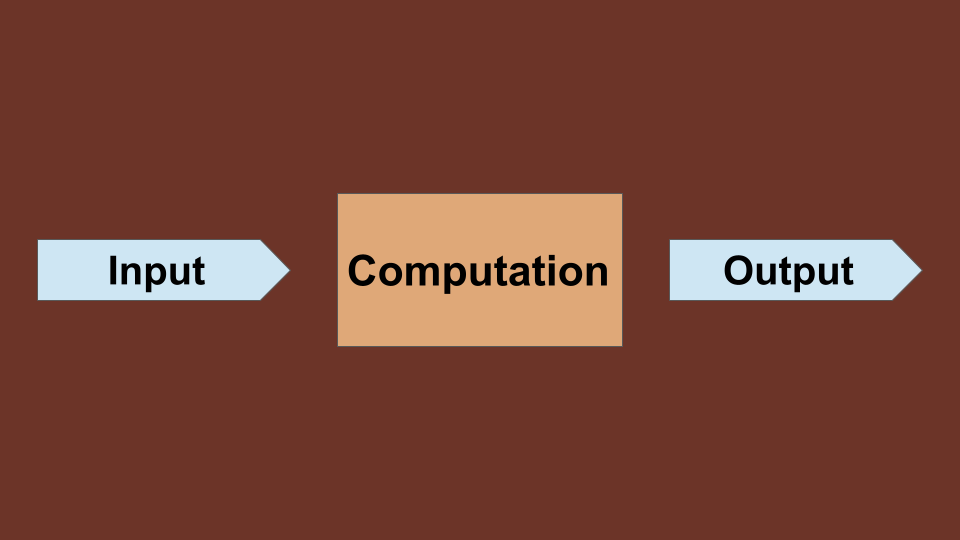
\includegraphics[width=0.8\textwidth]{standard computation model.png}
	\caption{یک واحد محاسباتی که مقادیری را به عنوان ورودی گرفته، پردازش کرده و سپس مقدار/مقادیر خروجی را ارائه کرده است.}
\end{figure}


در تصویر بالا یک نمود ساده از کامپیوتر‌های امروزی ارائه شده است. در دنیای واقعی مقدار ورودی می‌تواند از هر منبعی‌ تأمین شده باشد. با این وجود هدف ما بررسی منابع تولید ورودی نیست؛‌ بلکه هدف بررسی مقادیر ورودی (به صورت ایزوله) می‌باشد. می‌توان درنظر گرفت که ورودی داده شده و خروجی نهایی،‌هر دو در قالب یک رشته از اعداد باینری، ماتریس و یا هرقالب مدنظر کاربر باشند.

مهم‌ترین نکته درباره‌ی این واحد محاسباتی،‌ \textbf{در دسترس بودن کل مقادیر ورودی برای واحد پردازش} است. به عبارت دیگر\textbf{ واحد پردازش می‌تواند تمامی مقادیر ورودی را دریافت کرده و تشخیص} دهد. 

\subsection{مدل کوئری}
در مدل کوئری، داده‌های ورودی توسط یک تابع تولید می‌شوند. واحد محاسباتی دسترسی به تابع تولیدورودی دارد و می‌تواند برای دریافت داده‌های جدید،‌از تابع یاد شده،‌درخواست کند.

\begin{figure}[ht]
	\centering
	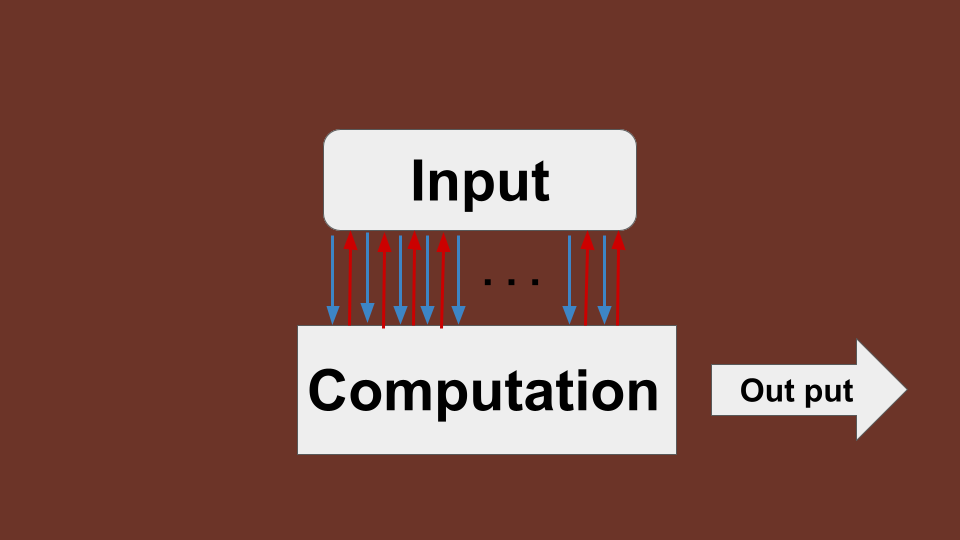
\includegraphics[width=0.8\textwidth]{Query computation model.png}
	\caption{شکل بالا نمود مدل محاسباتی‌کوئری است. واحد محاسباتی برای دریافت داده‌های جدید نیاز به درخواست از تابع \lr{input} دارد. خطوط قرمز و روبه‌بالا نشان از درخواست واحد محاسباتی و خطوط آبی روبه‌پایین نشان از پاسخ واحد \lr{input}می‌باشد.}
\end{figure}


در این مدل واحد محاسباتی دیگر داده‌ها را در قالب رشته‌ای از اطلاعات دردسترس ندارد؛ بلکه می‌تواند آن‌ها را از بخش \lr{input} دریافت کند. در گاهی از مواقع به سیستم \lr{input}،‌\lr{oracle} یا جعبه‌ی سیاه می‌گویند. تابع \lr{Oracle } یا جعبه‌ی سیاه یک سیستم است که ما به عنوان ناظر به سازوکار داخلی آن و  تمامی اطلاعات آن دسترسی نداریم و فقط می‌توانیم مقادیر مجاز را به آن داده و مقادیر خروجی را دریافت کنیم. 

تابع \lr{oracle} به صورت زیر تعریف می‌شود:
\begin{center}
$$
\left\{
\begin{array}{ll}
f : \sum^n = \sum^m\\
Which : m, n \in \mathbb{N}
\end{array}
\right.
$$
\end{center}

ما در این نظریه کوئری‌ها را می‌شماریم و وضعیت آن‌‌ها را بررسی می‌کنیم.

\section*{الگوریتم‌های کوانتومی}


%https://learn.qiskit.org/course/algorithms/query-algorithms#query-3-0
%https://www.youtube.com/watch?v=mGqyzZ-fnnY
%https://www.youtube.com/watch?v=CIq0PUkFDBc
%https://www.youtube.com/watch?v=7MdEHsRZxvo
%https://learn.qiskit.org/course/algorithms/query-algorithms#query-3-77
%https://learn.qiskit.org/course/algorithms/query-algorithms#query-5-0
%https://learn.qiskit.org/course/algorithms/query-algorithms#query-19-0
%https://www.youtube.com/watch?v=hK6BBluTGhU&list=PLay4zC7VCXV4gWb0ucSUQiGcRJFYMzROT&index=5
	
\section{Deutsch Algorithm}
\subsection{مسئله‌ی دوچ}
الگوریتم \lr{Deutsch} اولین و ساده‌ترین الگوریتم کوانتومی‌ است. این الگوریتم برای اولین بار در سال 1985 در مقاله‌ای مطرح شد؛ که توسط دیوید دوچ\footnote{David Deutsch} نوشته شده‌‌بود. این الگوریتم نقطه‌ی شروعی برای اثبات برتری کامپیوترهای کوانتومی نسبت به کامپوترهای کلاسیک است.

مسئله‌ی \lr{Deutsch} یکی از ساده‌ترین مفاهیم ممکن را مطرح می‌کند. اگر یک تابع به فرم زیر تعریف شود: 
\begin{center}
	$f : \sum \rightarrow \sum$
\end{center}
هدف بررسی ثابت بودن یا متعادل\footnote{Constante or balanse.} بودن تابع \lr{f} است. 
به‌طور کلی، درساده‌ترین حالت، می‌توان چهار وضعیت را برای تابع $f : \sum \rightarrow \sum$ درنظر گرفت:\\
\begin{figure}[ht]
	\centering
	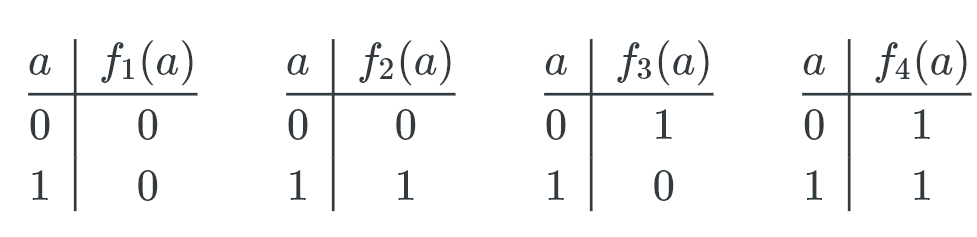
\includegraphics[width=0.8\textwidth]{Constantorbalanse.png}
	\caption{}
\end{figure}\\
در شکل بالا توابع \lr{f 1} , \lr{f 4} توابع ثابت و توابع \lr{f 2} و \lr{f 3} توابع متعادل هستند.
\begin{center}
\begin{tabular}{|c|c|}
	\hline
	\multicolumn{2}{|c|}{مسئله‌ی دوچ} \\
	\hline
	$f : \sum \rightarrow \sum$ & ورودی \\
	\hline
	صفر اگر تابع ثابت بود؛ یک اگر تابع متعادل بود.  & خروجی \\
	\hline
\end{tabular}
\end{center}
در الگوریتم‌های کلاسیک برای حل این مسئله، حداقل دو حالت باید بررسی شود.
\subsection{الگوریتم دوچ}
% https://www.youtube.com/watch?v=2wticzHE1vs&t=2014s
حال به بررسی الگوریتم دوچ می‌پردازیم. الگوریتمی که مسئله‌ی دوچ را با یک مدار کوانتومی حل می‌کند:\\
\begin{center}
\begin{figure}[ht]
	\centering
	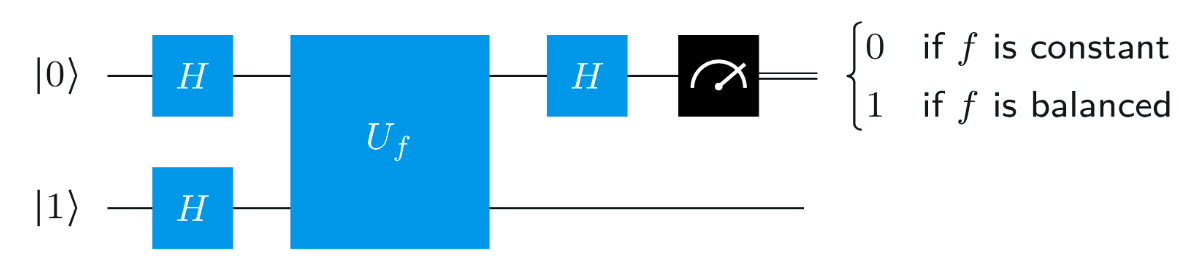
\includegraphics[width=0.8\textwidth]{Deutsch algorithm.png}
	\caption{}
\end{figure}
\end{center}


$$
\begin{aligned}
	\left|\pi_1\right\rangle= & |-\rangle|+\rangle=\frac{1}{2}(|0\rangle-|1\rangle)|0\rangle+\frac{1}{2}(|0\rangle-|1\rangle)|1\rangle \\
	\left|\pi_2\right\rangle= & \frac{1}{2}(|0 \oplus f(0)\rangle-|1 \oplus f(0)\rangle)|0\rangle+\frac{1}{2}(|0 \oplus f(1)\rangle-|1 \oplus f(1)\rangle)|1\rangle \\
	= & \frac{1}{2}(-1)^{f(0)}(|0\rangle-|1\rangle)|0\rangle+\frac{1}{2}(-1)^{f(1)}(|0\rangle-|1\rangle)|1\rangle \\
	& |0 \oplus a\rangle-|1 \oplus a\rangle=(-1)^a(|0\rangle-|1\rangle)
\end{aligned}
$$

$$
\begin{aligned}
	\left|\pi_1\right\rangle & =|-\rangle|+\rangle=\frac{1}{2}(|0\rangle-|1\rangle)|0\rangle+\frac{1}{2}(|0\rangle-|1\rangle)|1\rangle \\
	\left|\pi_2\right\rangle & =\frac{1}{2}(|0 \oplus f(0)\rangle-|1 \oplus f(0)\rangle)|0\rangle+\frac{1}{2}(|0 \oplus f(1)\rangle-|1 \oplus f(1)\rangle)|1\rangle \\
	& =\frac{1}{2}(-1)^{f(0)}(|0\rangle-|1\rangle)|0\rangle+\frac{1}{2}(-1)^{f(1)}(|0\rangle-|1\rangle)|1\rangle \\
	& =|-\rangle\left(\frac{(-1)^{f(0)}|0\rangle+(-1)^{f(1)}|1\rangle}{\sqrt{2}}\right)
\end{aligned}
$$

$$
\begin{aligned}
	\left|\pi_2\right\rangle & =|-\rangle\left(\frac{(-1)^{f(0)}|0\rangle+(-1)^{f(1)}|1\rangle}{\sqrt{2}}\right) \\
	& =(-1)^{f(0)}|-\rangle\left(\frac{|0\rangle+(-1)^{f(0) \oplus f(1)}|1\rangle}{\sqrt{2}}\right) \\
	& = \begin{cases}(-1)^{f(0)}|-\rangle|+\rangle & f(0) \oplus f(1)=0 \\
		(-1)^{f(0)}|-\rangle|-\rangle & f(0) \oplus f(1)=1\end{cases}
\end{aligned}
$$


$$
\begin{aligned}
	\left|\pi_2\right\rangle & = \begin{cases}(-1)^{f(0)}|-\rangle|+\rangle & f(0) \oplus f(1)=0 \\
		(-1)^{f(0)}|-\rangle|-\rangle & f(0) \oplus f(1)=1\end{cases} \\
	\left|\pi_3\right\rangle & = \begin{cases}(-1)^{f(0)}|-\rangle|0\rangle & f(0) \oplus f(1)=0 \\
		(-1)^{f(0)}|-\rangle|1\rangle & f(0) \oplus f(1)=1\end{cases} \\
	& =(-1)^{f(0)}|-\rangle|f(0) \oplus f(1)\rangle
\end{aligned}
$$

$$
\left|\pi_3\right\rangle=(-1)^{f(0)}|-\rangle|f(0) \oplus f(1)\rangle
$$
توضیحات رو بنویس



\newpage
\section{phase kickback}
% https://www.youtube.com/watch?v=2wticzHE1vs&t=2014s

$$
\begin{gathered}
	|b \oplus c\rangle=X^c|b\rangle \\
	u_f(|b\rangle|a\rangle)=|b \oplus f(a)\rangle|a\rangle=\left(X^{f(a)}|b\rangle\right)|a\rangle
\end{gathered}
$$

$$
\begin{aligned}
	\mathrm{U}_f(|b\rangle|a\rangle) & =\left(X^{f(a)}|b\rangle\right)|a\rangle \\
	U_f(|\psi\rangle|a\rangle) & =\left(X^{f(a)}|\psi\rangle\right)|a\rangle
\end{aligned}
$$

$$
\begin{gathered}
	u_f(|\psi\rangle|a\rangle)=\left(X^{f(a)}|\psi\rangle\right)|a\rangle \\
	u_f(|-\rangle|a\rangle)=\left(X^{f(a)}|-\rangle\right)|a\rangle=(-1)^{f(a)}|-\rangle|a\rangle \\
	X|-\rangle=-|-\rangle
\end{gathered}
$$
$$
\begin{aligned}
	\mathrm{U}_{\mathrm{f}} & (|-\rangle|\mathrm{a}\rangle)=(-1)^{\mathrm{f}(\mathrm{a})}|-\rangle|\mathrm{a}\rangle \longleftarrow \begin{array}{l}
		\text { phase } \\
		\text { kickback }
	\end{array} \\
	\left|\pi_1\right\rangle & =|-\rangle|+\rangle \\
	\left|\pi_2\right\rangle & =\mathrm{U}_{\mathrm{f}}(|-\rangle|+\rangle)=\frac{1}{\sqrt{2}} \mathrm{U}_{\mathrm{f}}(|-\rangle|0\rangle)+\frac{1}{\sqrt{2}} \mathrm{U}_{\mathrm{f}}(|-\rangle|1\rangle) \\
	& =|-\rangle\left(\frac{(-1)^{f(0)}|0\rangle+(-1)^{f(1)}|1\rangle}{\sqrt{2}}\right)
\end{aligned}
$$
\section{Deutsch-Jozsa Algorithm}




% https://www.youtube.com/watch?v=DyINHZoOcLQ
%https://www.youtube.com/watch?v=LTftC-eTLM0SS
--------------	
	
	
	
%computer vs simulator https://www.youtube.com/watch?v=2qcvgXaDdfU
% https://www.youtube.com/watch?v=0RPFWZj7Jm0	
	

\chapter{شبیه‌سازی پدیده‌های کوانتومی}
\section{Bell states}
در این بخش قصد داریم به بررسی پروتکل‌های ابتدایی در نظریه‌ی اطلاعات کوانتومی بپردازیم. تمامی این پروتکل‌ها به تعداد کمی کیوبیت نیاز دارند:؛ و در آزمایشگاه به صورت تجربی پیاده‌سازی شده‌اند. در اغلب موارد، سیستم از دو کیوبیت درهمتنیده تشکیل شده‌است. تابع حالت این سیستم‌ها به شکل زیر تعریف می‌شوند:
\begin{center}
	$\vert \psi_{00} \rangle = \frac{1}{\sqrt{2}}(|00\rangle + |11\rangle)$
\end{center}
برای آماده‌سازی این حالت کوانتومی‌، در حالت \lr{$\vert0\rangle$} داریم. با اعمال یک گیت هدامارد روی یکی از کیوبیت‌ها و سپس با کنترل‌ آن با گیت \lr{CNOT}، (به نحوی که کیوبیت دوم هدف قرارگیرد.) می‌توان به یک حالت درهمتنیده رسید. می‌توان این مراحل را به شکل زیر شرح داد:
\[
\vert\psi{00}\rangle = C_{10}H_{1}\vert00\rangle
\]

%می‌توان رابطه‌ی بالا را به هریک از حالات $\vert00\rangle, \vert 01\rangl, \vert 10\rangl, \vert 11\rangl$ تعمیم داد:%
\[
\vert\psi{xy}\rangle = C_{10}H_{1}\vert xy \rangle
\]

از آنجایی که چهار حالت |xy〉 یک مجموعه orthonormal هستند و دروازه‌های Hadamard و cNOT واحدی هستند، چهار حالت درهم تنیده |ψxy〉 نیز یک مجموعه orthonormal هستند، که به نام پایه Bell نامگذاری شده‌اند. حال یک دسته‌ی سه‌کیوبیتی را درنظر ‌می‌گیریم:



\section{entanglement}
\section{super dense coding}
\section{Teleport}
	
	

how to determine a oracle
-------------------
Bell state
superdencse coding
teleport

	
	
	
	
% https://learn.qiskit.org/course/ch-algorithms/quantum-circuits
	
	
	
\end{document}